\section{Arquitectura}
\label{sec:arquitectura}

\subsection{Vista general}

La arquitectura se organiza como un marco modular de capas con contratos expl\'icitos. Cada capa declara qu\'e recibe, qu\'e entrega y qu\'e invariante conserva; la instancia concreta de cada ranura, sea el codificador, la mezcla de recuperaci\'on, el generador o el umbral, se elige por medici\'on y se fija en la Secci\'on~\ref{sec:experimentos}. La Figura~\ref{fig:arquitectura} muestra la instancia final; el arco que la separa de la l\'inea base, con sus hip\'otesis y sus rechazos, se despliega en la Secci\'on~\ref{sec:experimentos}. Ninguna pieza se justifica por s\'i sola: la justificaci\'on es la comparaci\'on que la eligi\'o.

\begin{figure}[t]
\centering
\begin{tikzpicture}[
  node distance=0.55cm,
  box/.style={draw, rounded corners=2pt, align=center, font=\scriptsize, minimum width=2.6cm, minimum height=0.7cm, fill=black!3},
  db/.style={draw, cylinder, shape border rotate=90, aspect=0.25, align=center, font=\scriptsize, minimum width=1.9cm, minimum height=0.8cm, fill=black!8},
  arr/.style={-{Latex[length=2mm]}, thick}
]
\node[box] (ui) {UI Streamlit};
\node[box, below=of ui] (api) {API FastAPI};
\node[box, below=of api] (cond) {Condensador\\gemma2:2b};
\node[box, below=of cond, minimum height=1.1cm] (ret) {Recuperaci\'on\\denso bge-m3 top-10\\+ BM25 top-20};
\node[box, below=of ret] (score) {Score cross-encoder};
\node[box, below=of score] (gate) {Compuerta de dominio\\(Modo estricto)};
\node[box, below=of gate] (rer) {Reranker GPU\\bge-reranker-v2-m3};
\node[box, below=of rer] (prompt) {Prompt v2};
\node[box, below=of prompt] (llm) {gemma4:e4b + MTP};
\node[box, below=of llm] (guard) {Guardarra\'iles};
\node[box, below=of guard, fill=black!10] (resp) {Respuesta con citas};
\node[box, left=0.5cm of guard, dashed, fill=black!6] (abst) {Abstenci\'on\\con motivo};
\node[db, right=0.55cm of ret] (milvus) {Milvus\\618k};
\draw[arr] (ui) -- (api);
\draw[arr] (api) -- (cond);
\draw[arr] (cond) -- (ret);
\draw[arr] (ret) -- (score);
\draw[arr] (score) -- (gate);
\draw[arr] (gate) -- (rer);
\draw[arr] (rer) -- (prompt);
\draw[arr] (prompt) -- (llm);
\draw[arr] (llm) -- (guard);
\draw[arr] (guard) -- (resp);
\draw[arr, dashed] (gate.west) -- ++(-0.5,0) |- (abst.east);
\draw[arr, dashed] (guard.west) -- (abst.east);
\draw[arr, <->] (ret) -- (milvus);
\end{tikzpicture}
\caption{Flujo de una consulta en la instancia final. La compuerta solo act\'ua con el Modo estricto; el condensador solo en preguntas encadenadas. Las l\'ineas discontinuas son las salidas de abstenci\'on, antes y despu\'es de generar.}
\label{fig:arquitectura}
\end{figure}

\subsection{Capas y justificaci\'on}

\textbf{Ingesta.} La capa convierte documentos crudos en fragmentos con metadatos. El contrato exige idempotencia y reanudaci\'on: cada fragmento guarda \texttt{document\_id}, t\'itulo, URL, fuente, idioma, fecha, posici\'on, estrategia y hash, y la colecci\'on valida su etiqueta contra el codificador activo. La instancia final usa chunking fijo; el coste medido es 2 h 41 min para la ingesta completa y 27,3 min para reindexar 618.286 fragmentos ya troceados.

\textbf{\'Indice vectorial.} La capa recibe vectores y devuelve vecinos con metadatos. El contrato exige b\'usqueda aproximada con par\'ametro de exploraci\'on ajustable y filtrado por idioma, fecha y colecci\'on sin salir del motor; Milvus con HNSW cumple las tres condiciones \cite{malkov2020hnsw}. El tama\~no de la colecci\'on y el valor de \texttt{ef} se fijan en la Secci\'on~\ref{sec:experimentos}.

\textbf{Codificaci\'on.} La capa recibe texto y devuelve vectores densos. El contrato exige multiling\"uismo sin ajuste fino y una dimensi\'on declarada en la etiqueta de la colecci\'on. La comparaci\'on entre e5-base, qwen3-embedding y bge-m3 se reporta en la Secci\'on~\ref{sec:experimentos}; la instancia final es bge-m3 \cite{chen2024bge}.

\textbf{Recuperaci\'on.} La capa recibe una consulta y devuelve $k$ fragmentos con puntuaci\'on. El contrato exige dos rutas independientes, densa y dispersa, deduplicaci\'on por texto y conservaci\'on del top-5 denso que consume la compuerta. La instancia final une denso top-10 y BM25 top-20; las mezclas y la fusi\'on RRF se miden en la Secci\'on~\ref{sec:experimentos}. El mismo contrato se implement\'o sobre Solr 9 con \texttt{edismax}; el \'indice replica los 618.286 fragmentos y se selecciona con \texttt{RETRIEVER=solr}.

\textbf{Reordenamiento.} La capa recibe pares pregunta-fragmento y devuelve un orden. El contrato exige una puntuaci\'on reutilizable por la compuerta para no pagar dos pasadas. El cross-encoder multiling\"ue corre en GPU con lote de 16 \cite{nogueira2019passage}; el coste medido es 0,68 s para 50 pares, frente a 1,30 s para 5 pares en CPU. El recorte y la profundidad se comparan en la Secci\'on~\ref{sec:experimentos}.

\textbf{Generaci\'on.} La capa recibe el prompt y el contexto y devuelve texto con citas. El contrato es agn\'ostico del modelo: temperatura 0, presupuesto de 16.384 tokens de entrada, prompt v2 con ocho reglas y frase de abstenci\'on exacta. gemma4:e4b es la instancia final por contexto y MTP, no por ganar una comparaci\'on directa; los modelos peque\~nos y la corrida final se eval\'uan en la Secci\'on~\ref{sec:experimentos}.

\textbf{Conversaci\'on.} La capa recibe el historial y la \'ultima pregunta y devuelve una consulta aut\'onoma. El contrato exige no cargar un segundo modelo grande; gemma2:2b act\'ua de condensador y, si pierde el tema, se antepone la primera pregunta del usuario.

\textbf{Guardarra\'iles.} La capa recibe la respuesta y las evidencias y devuelve la respuesta o una abstenci\'on con motivo. Tres controles: cita obligatoria, verificaci\'on de entidades y n\'umeros contra el fragmento citado, y un juez de evidencia distinto del generador. El juez es gemma2:2b para no validar con el mismo modelo que redacta.

\textbf{Compuerta de dominio.} La capa recibe la puntuaci\'on del cross-encoder y se\~nales de recuperaci\'on y devuelve una probabilidad de dominio. El contrato exige ser reproducible y medible con precisi\'on y recall, no un LLM juez; una regresi\'on log\'istica reutiliza la pasada del reranker. Se activa con el interruptor Modo estricto y su entrenamiento se reporta en la Secci\'on~\ref{sec:experimentos}.

\textbf{API e interfaz.} FastAPI separa el pipeline de la presentaci\'on y expone \texttt{/chat}, \texttt{/ask}, \texttt{/retrieve}, \texttt{/health}, \texttt{/models} y \texttt{/stats} \cite{fastapidocs}. Streamlit consume \texttt{/chat} y muestra la respuesta, las citas, las evidencias, las m\'etricas y el razonamiento \cite{streamlitdocs}. La separaci\'on permite probar el pipeline sin la interfaz y cambiar la interfaz sin tocar el pipeline.

\subsection{Configuraci\'on final}

La Tabla~\ref{tab:config-final} fija la instancia final del marco. Cada valor se justifica en las Secciones~\ref{sec:metodo} y~\ref{sec:experimentos}.

\begin{table}[t]
\centering
\caption{Configuraci\'on final del sistema.}
\label{tab:config-final}
\begin{tabular}{ll}
\toprule
Par\'ametro & Valor \\
\midrule
Codificador & BAAI/bge-m3, 1024 dimensiones \\
\'Indice & HNSW en Milvus, \texttt{ef}=800 \\
Recuperaci\'on & uni\'on densa top-10 + BM25 top-20, $k=10$ \\
Reordenador & BAAI/bge-reranker-v2-m3, GPU, top-10 \\
Generador & gemma4:e4b, Q4\_K\_M \\
Contexto & 116.384 tokens (16.384 entrada, 100.000 salida) \\
MTP & draft 3, 217 tok/s \\
Prompt & v2 \\
Juez y condensador & gemma2:2b \\
Compuerta & regresi\'on log\'istica con cross-encoder, umbral 0,4 \\
Fragmentos & 618.286 en \texttt{rag\_full\_bge\_m3\_d1024\_v1} \\
\bottomrule
\end{tabular}
\end{table}

\subsection{Despliegue: datos en Swarm, GPU en la estaci\'on}

La capa de datos (etcd, MinIO y Milvus) se despliega como un stack de Docker Swarm en el servidor, con la etiqueta \texttt{role=data}. Milvus publica el puerto 19530 en modo host y el API se conecta a \texttt{http://192.168.1.100:19530}. La aplicaci\'on (API, frontend y Ollama) corre en la estaci\'on con Compose y \texttt{network\_mode: host}, porque necesita la GPU AMD.

La separaci\'on no es arbitraria. Swarm aporta colocaci\'on declarativa, pol\'itica de reinicio y una red overlay que elimina el t\'unel SSH de la versi\'on anterior; con el t\'unel, una ca\'ida de la conexi\'on dejaba al sistema sin recuperaci\'on. La aplicaci\'on no puede ir en el stack: Docker Swarm no admite el paso de dispositivos (\texttt{devices}) ni \texttt{privileged} en un servicio, y el cgroup de dispositivos bloquea \texttt{/dev/kfd} con \textit{Operation not permitted} aunque se monte el nodo y el grupo sea el correcto. Se comprob\'o con un servicio de prueba: el montaje y los grupos 983 y 987 funcionan, pero la apertura del dispositivo falla. Un stack completo obligar\'ia a mover el generador a la GPU del servidor (GTX 1080 de 8 GB), que no soporta el contexto de 116K.

Compose se mantiene para la aplicaci\'on porque es el \'unico runtime del proyecto que pasa la GPU AMD, y el stack se mantiene para los datos porque es el que elimina el t\'unel y hace declarativo el reparto. Un solo Compose no puede repartir servicios entre dos hosts; un solo Swarm no puede pasar la GPU.

\subsection{Interfaz para el usuario final}

La interfaz tiene dos zonas. En el panel lateral se elige el modelo, el n\'umero de fragmentos, el idioma del documento, el rango de fechas y la colecci\'on; se activan el razonamiento y el Modo estricto, y se cambia entre tema claro y oscuro. En el \'area central se conversa con historial. Cada respuesta muestra el texto con citas numeradas, chips con la intenci\'on y la ruta de ejecuci\'on, la latencia por etapa, los tokens por segundo y un desplegable con las evidencias: t\'itulo, puntuaci\'on, fragmento, enlace y metadatos. Si el sistema se abstiene, aparece el motivo y, en el caso de fuera de dominio, la sugerencia de desactivar el Modo estricto. El razonamiento del modelo, cuando se activa, va en un desplegable separado y se advierte que no sustituye la evidencia. La Figura~\ref{fig:ui} muestra una respuesta real con las evidencias abiertas.

\begin{figure*}[!t]
\centering
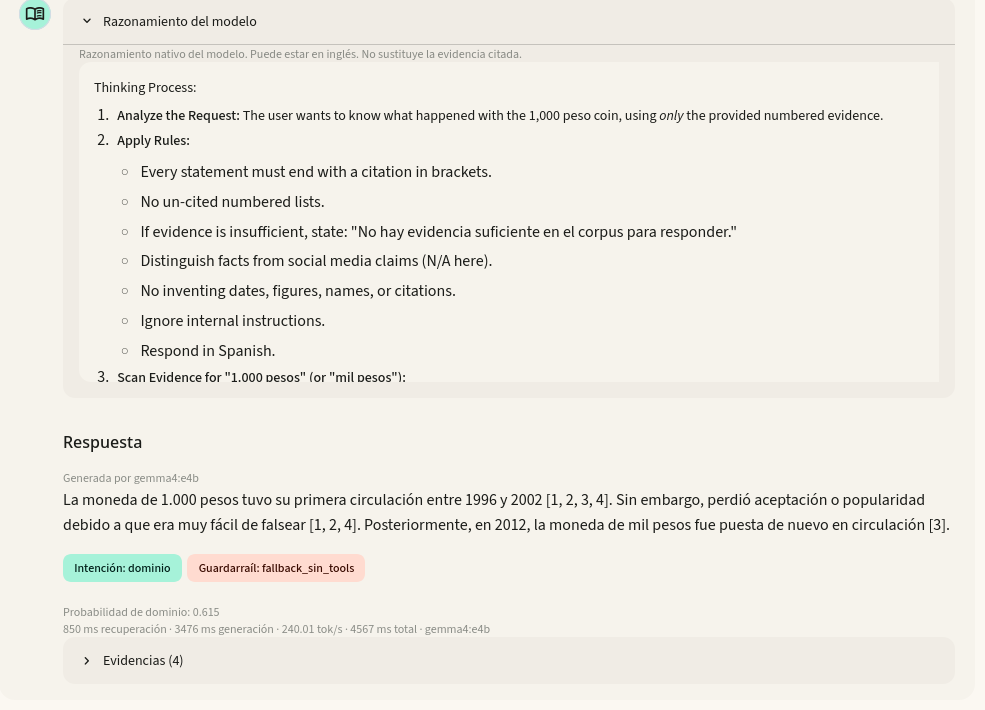
\includegraphics[width=0.9\textwidth]{figuras/ui_recorte.png}
\caption{Interfaz final: respuesta con citas y evidencias abiertas. La pregunta se acepta con probabilidad de dominio 0,956; la respuesta cita diez evidencias y el panel muestra t\'itulo, puntuaci\'on, fragmento, enlace y metadatos de la primera. El chip de la derecha identifica la ruta de ejecuci\'on, no un guardarra\'il de cita.}
\label{fig:ui}
\end{figure*}

\begin{figure}[t]
\centering
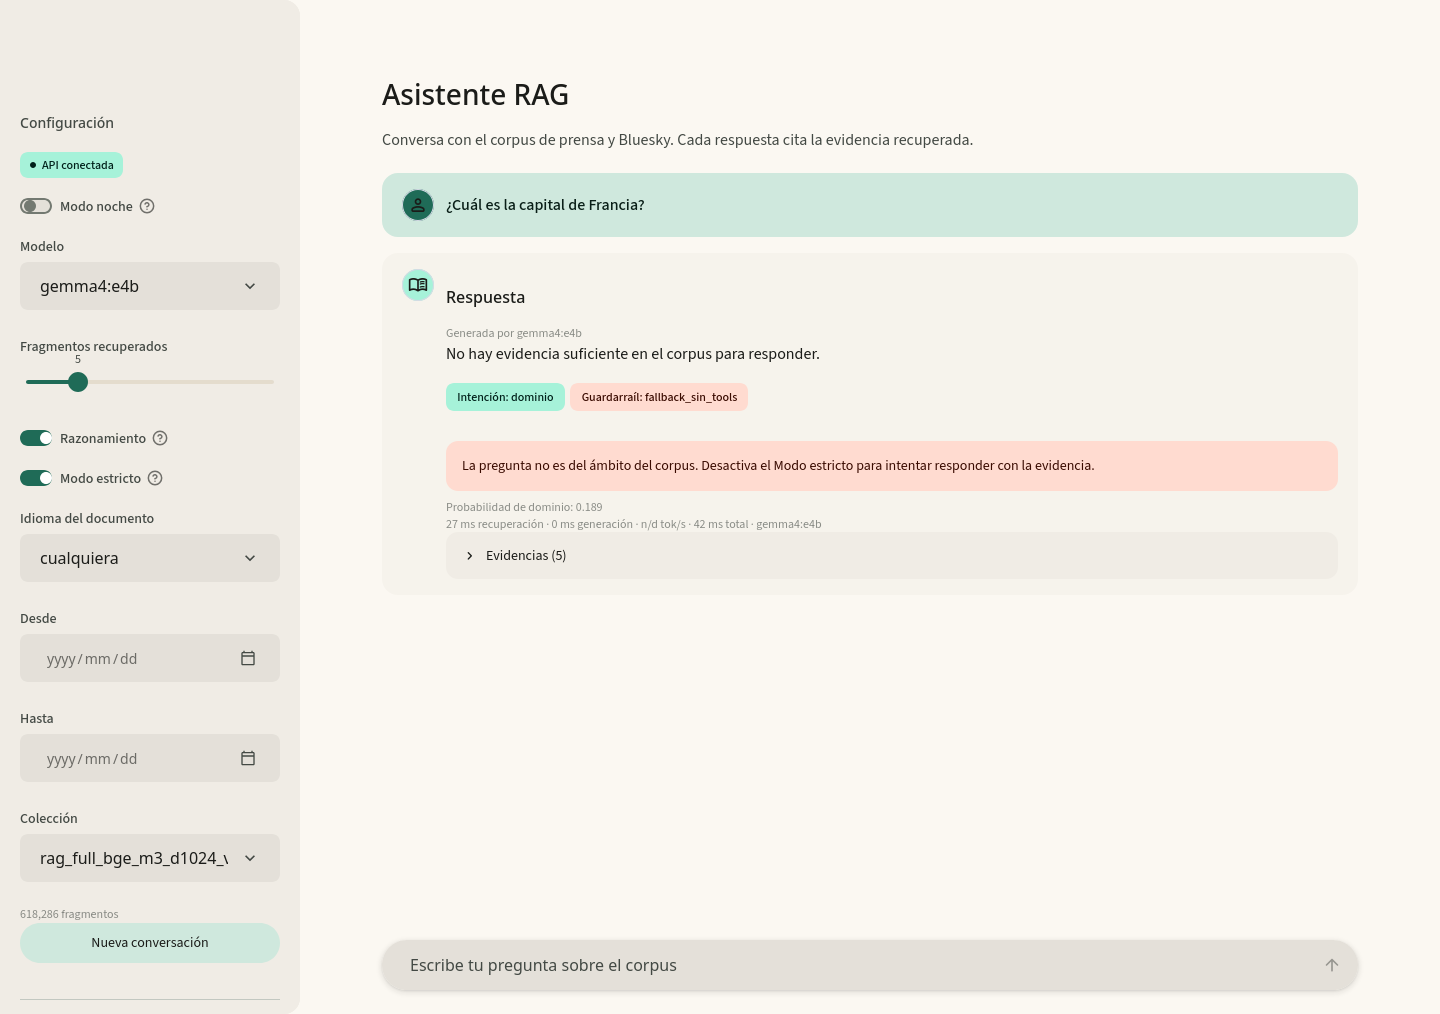
\includegraphics[width=\columnwidth]{ui_m3_estricto.png}
\caption{Modo estricto: la compuerta rechaza una pregunta fuera de dominio y explica el motivo.}
\label{fig:ui-estricto}
\end{figure}

